% Created by tikzDevice version 0.12.3.1 on 2022-11-29 12:40:03
% !TEX encoding = UTF-8 Unicode
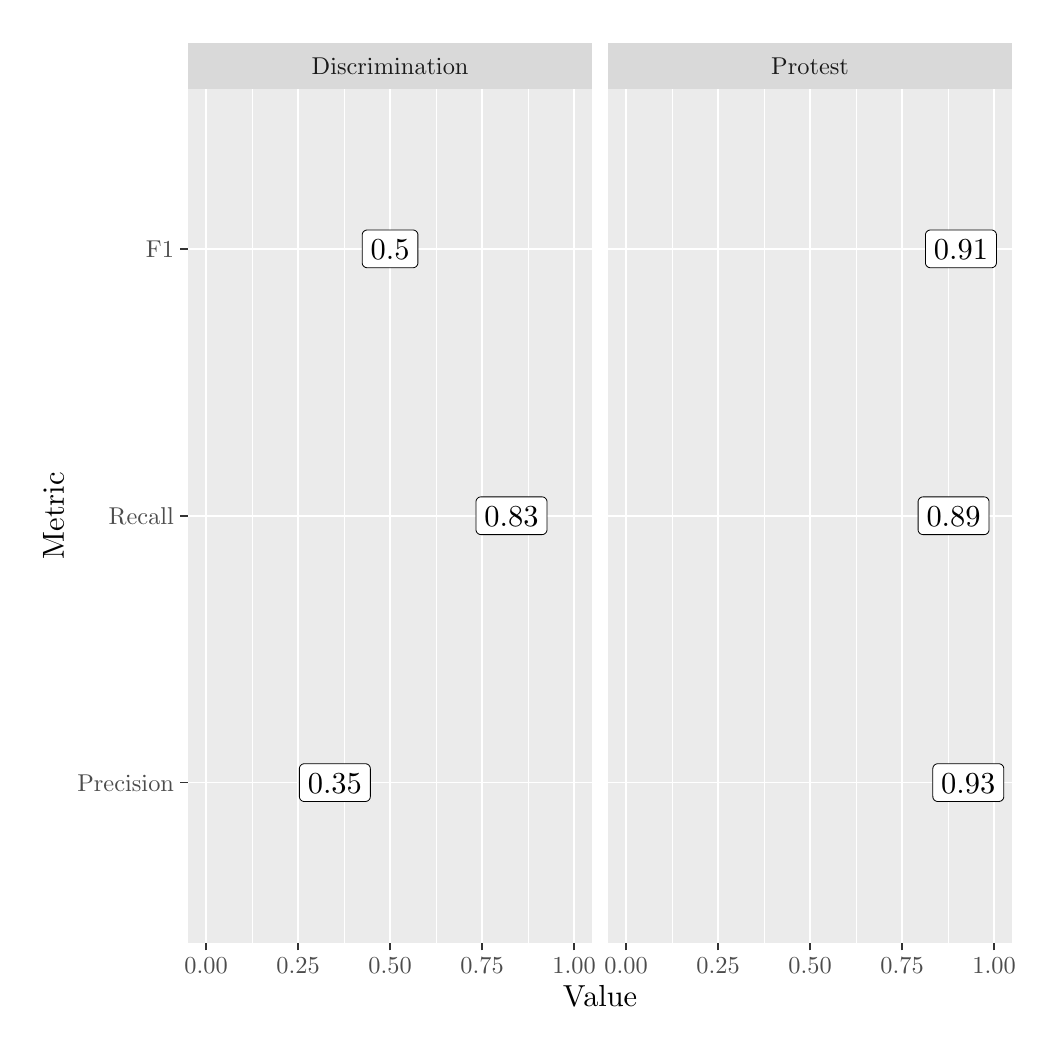
\begin{tikzpicture}[x=1pt,y=1pt]
\definecolor{fillColor}{RGB}{255,255,255}
\path[use as bounding box,fill=fillColor,fill opacity=0.00] (0,0) rectangle (361.35,361.35);
\begin{scope}
\path[clip] (  0.00,  0.00) rectangle (361.35,361.35);
\definecolor{drawColor}{RGB}{255,255,255}
\definecolor{fillColor}{RGB}{255,255,255}

\path[draw=drawColor,line width= 0.6pt,line join=round,line cap=round,fill=fillColor] (  0.00,  0.00) rectangle (361.35,361.35);
\end{scope}
\begin{scope}
\path[clip] ( 57.81, 30.69) rectangle (204.08,339.28);
\definecolor{fillColor}{gray}{0.92}

\path[fill=fillColor] ( 57.81, 30.69) rectangle (204.08,339.28);
\definecolor{drawColor}{RGB}{255,255,255}

\path[draw=drawColor,line width= 0.3pt,line join=round] ( 81.08, 30.69) --
	( 81.08,339.28);

\path[draw=drawColor,line width= 0.3pt,line join=round] (114.33, 30.69) --
	(114.33,339.28);

\path[draw=drawColor,line width= 0.3pt,line join=round] (147.57, 30.69) --
	(147.57,339.28);

\path[draw=drawColor,line width= 0.3pt,line join=round] (180.81, 30.69) --
	(180.81,339.28);

\path[draw=drawColor,line width= 0.6pt,line join=round] ( 57.81, 88.55) --
	(204.08, 88.55);

\path[draw=drawColor,line width= 0.6pt,line join=round] ( 57.81,184.98) --
	(204.08,184.98);

\path[draw=drawColor,line width= 0.6pt,line join=round] ( 57.81,281.42) --
	(204.08,281.42);

\path[draw=drawColor,line width= 0.6pt,line join=round] ( 64.46, 30.69) --
	( 64.46,339.28);

\path[draw=drawColor,line width= 0.6pt,line join=round] ( 97.70, 30.69) --
	( 97.70,339.28);

\path[draw=drawColor,line width= 0.6pt,line join=round] (130.95, 30.69) --
	(130.95,339.28);

\path[draw=drawColor,line width= 0.6pt,line join=round] (164.19, 30.69) --
	(164.19,339.28);

\path[draw=drawColor,line width= 0.6pt,line join=round] (197.43, 30.69) --
	(197.43,339.28);
\definecolor{drawColor}{RGB}{0,0,0}
\definecolor{fillColor}{RGB}{0,0,0}

\path[draw=drawColor,line width= 0.4pt,line join=round,line cap=round,fill=fillColor] (111.00, 88.55) circle (  3.57);

\path[draw=drawColor,line width= 0.4pt,line join=round,line cap=round,fill=fillColor] (174.83,184.98) circle (  3.57);

\path[draw=drawColor,line width= 0.4pt,line join=round,line cap=round,fill=fillColor] (130.95,281.42) circle (  3.57);
\definecolor{fillColor}{RGB}{255,255,255}

\path[draw=drawColor,line width= 0.3pt,line join=round,line cap=round,fill=fillColor] ( 99.99, 81.73) --
	(122.02, 81.73) --
	(121.94, 81.74) --
	(122.23, 81.75) --
	(122.52, 81.81) --
	(122.79, 81.91) --
	(123.04, 82.05) --
	(123.27, 82.24) --
	(123.46, 82.46) --
	(123.62, 82.70) --
	(123.73, 82.97) --
	(123.80, 83.25) --
	(123.82, 83.54) --
	(123.82, 83.54) --
	(123.82, 93.55) --
	(123.82, 93.55) --
	(123.80, 93.84) --
	(123.73, 94.13) --
	(123.62, 94.39) --
	(123.46, 94.64) --
	(123.27, 94.86) --
	(123.04, 95.04) --
	(122.79, 95.19) --
	(122.52, 95.29) --
	(122.23, 95.35) --
	(122.02, 95.36) --
	( 99.99, 95.36) --
	(100.20, 95.35) --
	( 99.91, 95.36) --
	( 99.62, 95.32) --
	( 99.35, 95.24) --
	( 99.08, 95.12) --
	( 98.84, 94.95) --
	( 98.63, 94.75) --
	( 98.46, 94.52) --
	( 98.32, 94.26) --
	( 98.23, 93.99) --
	( 98.18, 93.70) --
	( 98.18, 93.55) --
	( 98.18, 83.54) --
	( 98.18, 83.69) --
	( 98.18, 83.40) --
	( 98.23, 83.11) --
	( 98.32, 82.83) --
	( 98.46, 82.58) --
	( 98.63, 82.34) --
	( 98.84, 82.14) --
	( 99.08, 81.98) --
	( 99.35, 81.85) --
	( 99.62, 81.77) --
	( 99.91, 81.74) --
	cycle;
\end{scope}
\begin{scope}
\path[clip] ( 57.81, 30.69) rectangle (204.08,339.28);
\definecolor{drawColor}{RGB}{0,0,0}

\node[text=drawColor,anchor=base,inner sep=0pt, outer sep=0pt, scale=  1.10] at (111.00, 84.75) {0.35};
\definecolor{fillColor}{RGB}{255,255,255}

\path[draw=drawColor,line width= 0.3pt,line join=round,line cap=round,fill=fillColor] (163.81,178.17) --
	(185.84,178.17) --
	(185.77,178.17) --
	(186.06,178.18) --
	(186.35,178.24) --
	(186.62,178.34) --
	(186.87,178.49) --
	(187.09,178.67) --
	(187.29,178.89) --
	(187.44,179.14) --
	(187.56,179.40) --
	(187.63,179.69) --
	(187.65,179.98) --
	(187.65,179.98) --
	(187.65,189.99) --
	(187.65,189.99) --
	(187.63,190.28) --
	(187.56,190.56) --
	(187.44,190.83) --
	(187.29,191.07) --
	(187.09,191.29) --
	(186.87,191.48) --
	(186.62,191.62) --
	(186.35,191.72) --
	(186.06,191.78) --
	(185.84,191.80) --
	(163.81,191.80) --
	(164.03,191.78) --
	(163.74,191.79) --
	(163.45,191.76) --
	(163.17,191.68) --
	(162.91,191.55) --
	(162.67,191.39) --
	(162.46,191.19) --
	(162.29,190.95) --
	(162.15,190.70) --
	(162.06,190.42) --
	(162.01,190.13) --
	(162.01,189.99) --
	(162.01,179.98) --
	(162.01,180.12) --
	(162.01,179.83) --
	(162.06,179.54) --
	(162.15,179.27) --
	(162.29,179.01) --
	(162.46,178.78) --
	(162.67,178.58) --
	(162.91,178.41) --
	(163.17,178.29) --
	(163.45,178.21) --
	(163.74,178.17) --
	cycle;
\end{scope}
\begin{scope}
\path[clip] ( 57.81, 30.69) rectangle (204.08,339.28);
\definecolor{drawColor}{RGB}{0,0,0}

\node[text=drawColor,anchor=base,inner sep=0pt, outer sep=0pt, scale=  1.10] at (174.83,181.18) {0.83};
\definecolor{fillColor}{RGB}{255,255,255}

\path[draw=drawColor,line width= 0.3pt,line join=round,line cap=round,fill=fillColor] (122.69,274.60) --
	(139.20,274.60) --
	(139.13,274.61) --
	(139.42,274.62) --
	(139.71,274.68) --
	(139.98,274.78) --
	(140.23,274.92) --
	(140.45,275.11) --
	(140.65,275.33) --
	(140.80,275.57) --
	(140.92,275.84) --
	(140.99,276.12) --
	(141.01,276.41) --
	(141.01,276.41) --
	(141.01,286.42) --
	(141.01,286.42) --
	(140.99,286.71) --
	(140.92,287.00) --
	(140.80,287.26) --
	(140.65,287.51) --
	(140.45,287.73) --
	(140.23,287.91) --
	(139.98,288.06) --
	(139.71,288.16) --
	(139.42,288.22) --
	(139.20,288.23) --
	(122.69,288.23) --
	(122.91,288.22) --
	(122.62,288.23) --
	(122.33,288.19) --
	(122.05,288.11) --
	(121.79,287.99) --
	(121.55,287.82) --
	(121.34,287.62) --
	(121.16,287.39) --
	(121.03,287.13) --
	(120.94,286.86) --
	(120.89,286.57) --
	(120.88,286.42) --
	(120.88,276.41) --
	(120.89,276.56) --
	(120.89,276.27) --
	(120.94,275.98) --
	(121.03,275.70) --
	(121.16,275.45) --
	(121.34,275.21) --
	(121.55,275.01) --
	(121.79,274.85) --
	(122.05,274.72) --
	(122.33,274.64) --
	(122.62,274.61) --
	cycle;
\end{scope}
\begin{scope}
\path[clip] ( 57.81, 30.69) rectangle (204.08,339.28);
\definecolor{drawColor}{RGB}{0,0,0}

\node[text=drawColor,anchor=base,inner sep=0pt, outer sep=0pt, scale=  1.10] at (130.95,277.62) {0.5};
\end{scope}
\begin{scope}
\path[clip] (209.58, 30.69) rectangle (355.85,339.28);
\definecolor{fillColor}{gray}{0.92}

\path[fill=fillColor] (209.58, 30.69) rectangle (355.85,339.28);
\definecolor{drawColor}{RGB}{255,255,255}

\path[draw=drawColor,line width= 0.3pt,line join=round] (232.85, 30.69) --
	(232.85,339.28);

\path[draw=drawColor,line width= 0.3pt,line join=round] (266.09, 30.69) --
	(266.09,339.28);

\path[draw=drawColor,line width= 0.3pt,line join=round] (299.34, 30.69) --
	(299.34,339.28);

\path[draw=drawColor,line width= 0.3pt,line join=round] (332.58, 30.69) --
	(332.58,339.28);

\path[draw=drawColor,line width= 0.6pt,line join=round] (209.58, 88.55) --
	(355.85, 88.55);

\path[draw=drawColor,line width= 0.6pt,line join=round] (209.58,184.98) --
	(355.85,184.98);

\path[draw=drawColor,line width= 0.6pt,line join=round] (209.58,281.42) --
	(355.85,281.42);

\path[draw=drawColor,line width= 0.6pt,line join=round] (216.23, 30.69) --
	(216.23,339.28);

\path[draw=drawColor,line width= 0.6pt,line join=round] (249.47, 30.69) --
	(249.47,339.28);

\path[draw=drawColor,line width= 0.6pt,line join=round] (282.72, 30.69) --
	(282.72,339.28);

\path[draw=drawColor,line width= 0.6pt,line join=round] (315.96, 30.69) --
	(315.96,339.28);

\path[draw=drawColor,line width= 0.6pt,line join=round] (349.20, 30.69) --
	(349.20,339.28);
\definecolor{drawColor}{RGB}{0,0,0}
\definecolor{fillColor}{RGB}{0,0,0}

\path[draw=drawColor,line width= 0.4pt,line join=round,line cap=round,fill=fillColor] (339.89, 88.55) circle (  3.57);

\path[draw=drawColor,line width= 0.4pt,line join=round,line cap=round,fill=fillColor] (334.57,184.98) circle (  3.57);

\path[draw=drawColor,line width= 0.4pt,line join=round,line cap=round,fill=fillColor] (337.23,281.42) circle (  3.57);
\definecolor{fillColor}{RGB}{255,255,255}

\path[draw=drawColor,line width= 0.3pt,line join=round,line cap=round,fill=fillColor] (328.88, 81.73) --
	(350.91, 81.73) --
	(350.84, 81.74) --
	(351.13, 81.75) --
	(351.41, 81.81) --
	(351.68, 81.91) --
	(351.94, 82.05) --
	(352.16, 82.24) --
	(352.35, 82.46) --
	(352.51, 82.70) --
	(352.62, 82.97) --
	(352.69, 83.25) --
	(352.72, 83.54) --
	(352.72, 83.54) --
	(352.72, 93.55) --
	(352.72, 93.55) --
	(352.69, 93.84) --
	(352.62, 94.13) --
	(352.51, 94.39) --
	(352.35, 94.64) --
	(352.16, 94.86) --
	(351.94, 95.04) --
	(351.68, 95.19) --
	(351.41, 95.29) --
	(351.13, 95.35) --
	(350.91, 95.36) --
	(328.88, 95.36) --
	(329.10, 95.35) --
	(328.81, 95.36) --
	(328.52, 95.32) --
	(328.24, 95.24) --
	(327.97, 95.12) --
	(327.74, 94.95) --
	(327.53, 94.75) --
	(327.35, 94.52) --
	(327.22, 94.26) --
	(327.12, 93.99) --
	(327.08, 93.70) --
	(327.07, 93.55) --
	(327.07, 83.54) --
	(327.08, 83.69) --
	(327.08, 83.40) --
	(327.12, 83.11) --
	(327.22, 82.83) --
	(327.35, 82.58) --
	(327.53, 82.34) --
	(327.74, 82.14) --
	(327.97, 81.98) --
	(328.24, 81.85) --
	(328.52, 81.77) --
	(328.81, 81.74) --
	cycle;
\end{scope}
\begin{scope}
\path[clip] (209.58, 30.69) rectangle (355.85,339.28);
\definecolor{drawColor}{RGB}{0,0,0}

\node[text=drawColor,anchor=base,inner sep=0pt, outer sep=0pt, scale=  1.10] at (339.89, 84.75) {0.93};
\definecolor{fillColor}{RGB}{255,255,255}

\path[draw=drawColor,line width= 0.3pt,line join=round,line cap=round,fill=fillColor] (323.56,178.17) --
	(345.59,178.17) --
	(345.52,178.17) --
	(345.81,178.18) --
	(346.09,178.24) --
	(346.36,178.34) --
	(346.62,178.49) --
	(346.84,178.67) --
	(347.03,178.89) --
	(347.19,179.14) --
	(347.30,179.40) --
	(347.37,179.69) --
	(347.40,179.98) --
	(347.40,179.98) --
	(347.40,189.99) --
	(347.40,189.99) --
	(347.37,190.28) --
	(347.30,190.56) --
	(347.19,190.83) --
	(347.03,191.07) --
	(346.84,191.29) --
	(346.62,191.48) --
	(346.36,191.62) --
	(346.09,191.72) --
	(345.81,191.78) --
	(345.59,191.80) --
	(323.56,191.80) --
	(323.78,191.78) --
	(323.49,191.79) --
	(323.20,191.76) --
	(322.92,191.68) --
	(322.66,191.55) --
	(322.42,191.39) --
	(322.21,191.19) --
	(322.03,190.95) --
	(321.90,190.70) --
	(321.80,190.42) --
	(321.76,190.13) --
	(321.75,189.99) --
	(321.75,179.98) --
	(321.76,180.12) --
	(321.76,179.83) --
	(321.80,179.54) --
	(321.90,179.27) --
	(322.03,179.01) --
	(322.21,178.78) --
	(322.42,178.58) --
	(322.66,178.41) --
	(322.92,178.29) --
	(323.20,178.21) --
	(323.49,178.17) --
	cycle;
\end{scope}
\begin{scope}
\path[clip] (209.58, 30.69) rectangle (355.85,339.28);
\definecolor{drawColor}{RGB}{0,0,0}

\node[text=drawColor,anchor=base,inner sep=0pt, outer sep=0pt, scale=  1.10] at (334.57,181.18) {0.89};
\definecolor{fillColor}{RGB}{255,255,255}

\path[draw=drawColor,line width= 0.3pt,line join=round,line cap=round,fill=fillColor] (326.22,274.60) --
	(348.25,274.60) --
	(348.18,274.61) --
	(348.47,274.62) --
	(348.75,274.68) --
	(349.02,274.78) --
	(349.28,274.92) --
	(349.50,275.11) --
	(349.69,275.33) --
	(349.85,275.57) --
	(349.96,275.84) --
	(350.03,276.12) --
	(350.06,276.41) --
	(350.06,276.41) --
	(350.06,286.42) --
	(350.06,286.42) --
	(350.03,286.71) --
	(349.96,287.00) --
	(349.85,287.26) --
	(349.69,287.51) --
	(349.50,287.73) --
	(349.28,287.91) --
	(349.02,288.06) --
	(348.75,288.16) --
	(348.47,288.22) --
	(348.25,288.23) --
	(326.22,288.23) --
	(326.44,288.22) --
	(326.15,288.23) --
	(325.86,288.19) --
	(325.58,288.11) --
	(325.32,287.99) --
	(325.08,287.82) --
	(324.87,287.62) --
	(324.69,287.39) --
	(324.56,287.13) --
	(324.46,286.86) --
	(324.42,286.57) --
	(324.41,286.42) --
	(324.41,276.41) --
	(324.42,276.56) --
	(324.42,276.27) --
	(324.46,275.98) --
	(324.56,275.70) --
	(324.69,275.45) --
	(324.87,275.21) --
	(325.08,275.01) --
	(325.32,274.85) --
	(325.58,274.72) --
	(325.86,274.64) --
	(326.15,274.61) --
	cycle;
\end{scope}
\begin{scope}
\path[clip] (209.58, 30.69) rectangle (355.85,339.28);
\definecolor{drawColor}{RGB}{0,0,0}

\node[text=drawColor,anchor=base,inner sep=0pt, outer sep=0pt, scale=  1.10] at (337.23,277.62) {0.91};
\end{scope}
\begin{scope}
\path[clip] ( 57.81,339.28) rectangle (204.08,355.85);
\definecolor{fillColor}{gray}{0.85}

\path[fill=fillColor] ( 57.81,339.28) rectangle (204.08,355.85);
\definecolor{drawColor}{gray}{0.10}

\node[text=drawColor,anchor=base,inner sep=0pt, outer sep=0pt, scale=  0.88] at (130.95,344.53) {Discrimination};
\end{scope}
\begin{scope}
\path[clip] (209.58,339.28) rectangle (355.85,355.85);
\definecolor{fillColor}{gray}{0.85}

\path[fill=fillColor] (209.58,339.28) rectangle (355.85,355.85);
\definecolor{drawColor}{gray}{0.10}

\node[text=drawColor,anchor=base,inner sep=0pt, outer sep=0pt, scale=  0.88] at (282.72,344.53) {Protest};
\end{scope}
\begin{scope}
\path[clip] (  0.00,  0.00) rectangle (361.35,361.35);
\definecolor{drawColor}{gray}{0.20}

\path[draw=drawColor,line width= 0.6pt,line join=round] ( 64.46, 27.94) --
	( 64.46, 30.69);

\path[draw=drawColor,line width= 0.6pt,line join=round] ( 97.70, 27.94) --
	( 97.70, 30.69);

\path[draw=drawColor,line width= 0.6pt,line join=round] (130.95, 27.94) --
	(130.95, 30.69);

\path[draw=drawColor,line width= 0.6pt,line join=round] (164.19, 27.94) --
	(164.19, 30.69);

\path[draw=drawColor,line width= 0.6pt,line join=round] (197.43, 27.94) --
	(197.43, 30.69);
\end{scope}
\begin{scope}
\path[clip] (  0.00,  0.00) rectangle (361.35,361.35);
\definecolor{drawColor}{gray}{0.30}

\node[text=drawColor,anchor=base,inner sep=0pt, outer sep=0pt, scale=  0.88] at ( 64.46, 19.68) {0.00};

\node[text=drawColor,anchor=base,inner sep=0pt, outer sep=0pt, scale=  0.88] at ( 97.70, 19.68) {0.25};

\node[text=drawColor,anchor=base,inner sep=0pt, outer sep=0pt, scale=  0.88] at (130.95, 19.68) {0.50};

\node[text=drawColor,anchor=base,inner sep=0pt, outer sep=0pt, scale=  0.88] at (164.19, 19.68) {0.75};

\node[text=drawColor,anchor=base,inner sep=0pt, outer sep=0pt, scale=  0.88] at (197.43, 19.68) {1.00};
\end{scope}
\begin{scope}
\path[clip] (  0.00,  0.00) rectangle (361.35,361.35);
\definecolor{drawColor}{gray}{0.20}

\path[draw=drawColor,line width= 0.6pt,line join=round] (216.23, 27.94) --
	(216.23, 30.69);

\path[draw=drawColor,line width= 0.6pt,line join=round] (249.47, 27.94) --
	(249.47, 30.69);

\path[draw=drawColor,line width= 0.6pt,line join=round] (282.72, 27.94) --
	(282.72, 30.69);

\path[draw=drawColor,line width= 0.6pt,line join=round] (315.96, 27.94) --
	(315.96, 30.69);

\path[draw=drawColor,line width= 0.6pt,line join=round] (349.20, 27.94) --
	(349.20, 30.69);
\end{scope}
\begin{scope}
\path[clip] (  0.00,  0.00) rectangle (361.35,361.35);
\definecolor{drawColor}{gray}{0.30}

\node[text=drawColor,anchor=base,inner sep=0pt, outer sep=0pt, scale=  0.88] at (216.23, 19.68) {0.00};

\node[text=drawColor,anchor=base,inner sep=0pt, outer sep=0pt, scale=  0.88] at (249.47, 19.68) {0.25};

\node[text=drawColor,anchor=base,inner sep=0pt, outer sep=0pt, scale=  0.88] at (282.72, 19.68) {0.50};

\node[text=drawColor,anchor=base,inner sep=0pt, outer sep=0pt, scale=  0.88] at (315.96, 19.68) {0.75};

\node[text=drawColor,anchor=base,inner sep=0pt, outer sep=0pt, scale=  0.88] at (349.20, 19.68) {1.00};
\end{scope}
\begin{scope}
\path[clip] (  0.00,  0.00) rectangle (361.35,361.35);
\definecolor{drawColor}{gray}{0.30}

\node[text=drawColor,anchor=base east,inner sep=0pt, outer sep=0pt, scale=  0.88] at ( 52.86, 85.52) {Precision};

\node[text=drawColor,anchor=base east,inner sep=0pt, outer sep=0pt, scale=  0.88] at ( 52.86,181.95) {Recall};

\node[text=drawColor,anchor=base east,inner sep=0pt, outer sep=0pt, scale=  0.88] at ( 52.86,278.39) {F1};
\end{scope}
\begin{scope}
\path[clip] (  0.00,  0.00) rectangle (361.35,361.35);
\definecolor{drawColor}{gray}{0.20}

\path[draw=drawColor,line width= 0.6pt,line join=round] ( 55.06, 88.55) --
	( 57.81, 88.55);

\path[draw=drawColor,line width= 0.6pt,line join=round] ( 55.06,184.98) --
	( 57.81,184.98);

\path[draw=drawColor,line width= 0.6pt,line join=round] ( 55.06,281.42) --
	( 57.81,281.42);
\end{scope}
\begin{scope}
\path[clip] (  0.00,  0.00) rectangle (361.35,361.35);
\definecolor{drawColor}{RGB}{0,0,0}

\node[text=drawColor,anchor=base,inner sep=0pt, outer sep=0pt, scale=  1.10] at (206.83,  7.64) {Value};
\end{scope}
\begin{scope}
\path[clip] (  0.00,  0.00) rectangle (361.35,361.35);
\definecolor{drawColor}{RGB}{0,0,0}

\node[text=drawColor,rotate= 90.00,anchor=base,inner sep=0pt, outer sep=0pt, scale=  1.10] at ( 13.08,184.98) {Metric};
\end{scope}
\end{tikzpicture}
